% $Id: gui_preproc.tex 395 2011-11-17 22:34:59Z cphillip $
%
% Written by Jessica Schrouff
%_______________________________________________

\chapter{Prepare feature set}
\label{chap:PrepFeat}
\minitoc

\section{Introduction}
%===============
\label{sec:prep_intro}
One of the main inputs of a machine learning algorithm consists in a $N_{samples} \times N_{features}$ data matrix, containing the feature values for each sample.  This matrix can either be input directly into the machine or be used to compute a `similarity matrix', or kernel, of size $N_{samples} \times N_{samples}$, which is then input into the classification/regression algorithm [see ``kernel trick" \cite{Hofmann2008,Aizerman1964}]. PRoNTo computes a linear kernel (i.e. dot product) between the samples. The `Prepare Feature Set' step computes both the features and linear kernel matrices from one or more modalities, as defined in the previously described `Data \& Design' module (see chapter \ref{chap:DataDesign}).  It allows detrending the features in the case of time series (such as fMRI) and scaling each image by a constant factor (input by the user) in the case of quantitative modalities (such as PET). Masks can be specified to select a subset of features for later modeling (e.g. Regions of Interest for MRI or fMRI data or electrodes/channes for M/EEG data).
\\

Multiple runs entered as different modalities (e.g. modality 1 is `fMRI\_run1', modality 2 is `fMRI\_run2',...) can be concatenated as samples during this step. In this case, the images from different runs should have the same number of features. In addition, from v2.0 one is allowed to build multiple kernels, either from multiple modalities, or based on different anatomically labelled regions as defined by an atlas. In case of multiple modalities, it is required that the selected modalities have the same number of samples.
\\

In ProNTo versions 2.X, modalities could be combined in 2 ways at this stage: either concatenated as samples (e.g. multiple runs of a same experiment), or combined as additional features by computing one kernel per modality and storing them together. This had the limitation that combined modalities (in either way) had to have the exact same number of features. From v3.0 we have decoupled those operations for more flexibility. At the feature set stage, different modalities can only be concatenated as samples. In this case they still need to have the exact same number of features.
\\[1cm]






\section{Feature extraction and pre-processing}
\label{sec:feat_extr}


In order to combine different types of modalities (or data) as different types of features in the predicted models from PRoNTo v3.0 it is necessary to build one feature set per modality. The different features sets can then be combined later on the model specification step, either added/concatenated or using MKL.
\\

In PRoNTo v3.0 the different data formats are handled in different ways: NIfTI images and .mat in a way similar to versions 2.X, while MEEG is handled differently through a new window. This means that now, you have to first load the `PRT.mat' in the `Prepare feature set' GUI in order for PRoNTo to track the different data formats that exist in your PRT. So after clicking on the `Prepare Feature Set' button in the main interface, a second window will appear first, allowing the user to select a saved PRT.mat. If it has more than one different data formats, figure \ref{fig:gui_prepare_featureSet_specify_data_type} will appear prompting you to choose the feature set's data format that you want to build. Feature sets are built for each specific data format at a time. The buttons available on this interface will reflect the data formats previously specified in the `Data \& Design' module. If only one type is present, this step is skipped and PRoNTo launches directly the main `Prepare feature set' window after the user has selected a saved PRT.mat.
\\

\begin{figure}[!h]
  \centering
		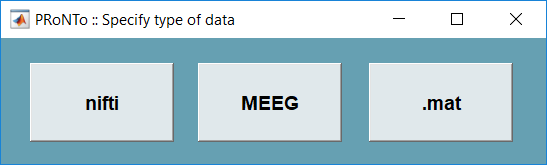
\includegraphics[scale=0.72]{images/Tutorial/v3/gui_prepare_featureSet_specify_data_type.png}
	\caption{`Specify type of data' GUI}
	\label{fig:gui_prepare_featureSet_specify_data_type}
\end{figure}

In case there are more than one data formats, \textbf{if the `nifti' option is selected} to be included in the feature set (further referred to as FS), the toolbox will extract information from the voxels/features contained within the first-level mask that was selected for that modality (mask specified at the `Data \& Design' step, see chapter `Data \& Design'). This is performed by extracting `blocks' of features, not to overload the RAM (Random-Access Memory). 
\\

\textbf{If the `MEEG' or the `.mat' options are selected}, as mentioned in the previous chapters, the data are assumed to have already been pre-processed to contain only the relevant features (and therefore there is no need for a mask), as this can be easily performed during pre-processing.
\\

In case of time-series data (e.g. fMRI), the user can specify detrending
methods and parameters to apply to the time course of each feature. Methods comprise a polynomial detrending (parameter: order of the polynomial) or
a Discrete Cosine Transform high-pass filter (SPM, parameter: frequency cutoff in seconds). An example of a linear detrending (polynomial detrending
of order 1) is shown in Fig. \ref{fig:lindetrend}.

\begin{figure}[!h]
  \begin{center}
      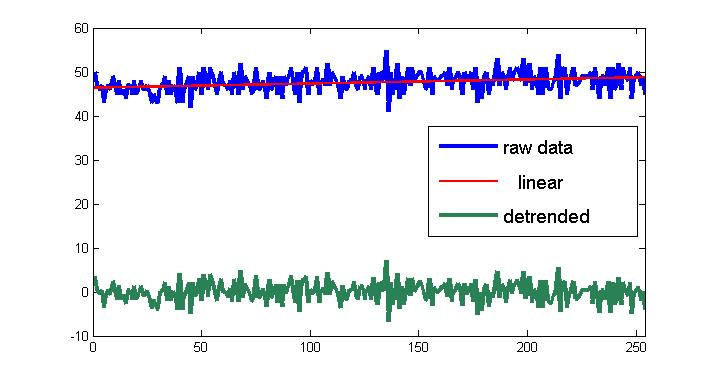
\includegraphics[height=6.2cm]{images/fig1_lindetrend.png}
   \caption{Example of detrending: the original signal over time of one feature (in blue) was approximated by a polynomial of order 1 (red line), which was then substracted from the original signal to give the detrended signal (in green).}
    \label{fig:lindetrend}
  \end{center}
\end{figure}


After you do that, the main `Prepare feature set' window will appear (Figure \ref{fig:FSmainl}), where you will be prompted to specify the name of the FS and to define the number of modalities which should be included in the FS.
\\

\begin{figure}[!h]
  \begin{center}
      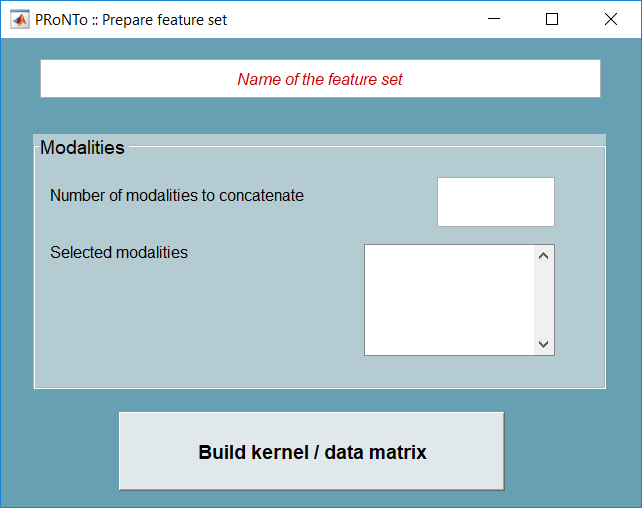
\includegraphics[height=7cm]{images/Tutorial/v3/prepare_feature_set.png}
   \caption{`Prepare feature set' GUI}
    \label{fig:FSmainl}
  \end{center}
\end{figure}


\noindent \textbf{Note:} If you have been using PRoNTo versions 2.X you will notice that the checkbox that used to be available and allowed to build one kernel per modality (if multiple modalities were present/had been selected in the FS) is not available anymore since from PRoNTo v3.0 different modalities can be combined at the model level.
\\

To define the number of modalities to include, the user should click in the appropriate edit box, type the number and then `enter'. This will launch a third window (Figure \ref{fig:modFS} for NIfTI and .mat, or Figure \ref{fig:gui_meeg_prepare_featureSet_specify_modality} for MEEG), allowing the specification of the different options and parameters for each modality. When the dataset contains only one modality, this window is launched directly and (Figure \ref{fig:FSmainl}) is filled automatically and only expect the feature set name. The two windows are further explained in the sections that follow.
\\



So for each modality, the features are then written in a file array (with a `.dat' extension) on the hard drive (in the same directory as the dataset). Please note that in the case of large datasets, this operation may require many Gb of free space on the hard drive and long computational times. Therefore, if the first condition can't be fulfilled, we recommend the use of external drives for the whole analysis. Regarding the computational expenses, we tried to minimize their effect by extracting/computing the features only once per modality: when preparing other feature sets using the same modality and detrending parameters, the built file array will be accessed for the next steps.
\\


{\bf Be careful} that using the same modality but different detrending (for NIfTI) or averaging (for MEEG) methods and/or parameters will force the re-computation of the file array for the considered modality. In the same way, changing the dataset ({\tt PRT.mat}) from directory might lead to the re-computation of the feature sets if the file arrays were not moved accordingly.  % From the feature set(s), a linear kernel can then be computed.







% USED ALREADY IN THE INTRO. USE ONLY THE \REFs
% To define the number of modalities to include, the user should click in the appropriate edit box, type the number and then `enter'. This will launch a third window (Figure \ref{fig:modFS} for NIfTI and .mat, or Figure \ref{fig:gui_meeg_prepare_featureSet_specify_modality} for MEEG), allowing the specification of the different options and parameters for each modality. When the dataset contains only one modality, this window is launched directly and (Fig. \ref{fig:FSmainl}) is filled automatically and only expect the feature set name.
% \\





\section{Prepare feature set}
After defining the name of the FS and also, in case of multiple data formats, the number of modalities to include, the `Specify modality' window is launched to allow the user to specify the different options and parameters for each modality.

\subsection{NIfTI and .mat data}
\label{ssec:feature_nifti_mat}

For NIfTI and .mat data formats, the window looks like figure \ref{fig:modFS}.
\\

\begin{figure}[!h]
  \begin{center}
      
\includegraphics[height=9cm]{images/Tutorial/v3/gui_prepare_featureSet_specify_modality.png}
   \caption{`Specify modality' GUI for NIfTI and .mat data.}
    \label{fig:modFS}
  \end{center}
\end{figure}

In this window the user has to first choose which modality to include based on its name (first pull-down menu) and  which conditions to use to build the kernel. In `all scans' the kernel matrix will be computed between all scans within the time series of all subjects and in `all conds' the kernel matrix is computed only between the scans corresponding to the specified conditions of interest (see `Data \& Design'). By default, the toolbox will use all scans to compute the kernel. With large datasets however, computational expenses can be reduced by selecting the last option. All other options are facultative.

\subsubsection{Parameters}

The first panel refers to operations to perform on the features:

\begin{itemize}

\item \textbf{Detrend:} By default, the parameter is set to `No detrending'. However, we recommend to perform a detrending in the case of time series data such as fMRI (and only in that case). When selecting polynomial, the `order' parameter will appear, with a default value of 1. Changing this value will increase the order of the polynomial used to fit the data. If `Discrete Cosine Transform' is selected, the editable parameter corresponds to the cutoff frequency (in seconds) of the high-pass filter. Please note that, when including more than one run (`modality') into a feature set, nothing will prevent the user from using different detrending methods/parameters. We however highly recommend to use a consistent detrending in the same FS. \textbf{Note:} Since .mat files are assumed to have been pre-processed prior to using them with PRoNTo, detrending is mainly required only for fMRI data.

\item \textbf{Scaling:} Allows the specification of constant values to scale each scan. `no scaling' is the default option. However, when dealing with quantitative modalities such as PET, the user should provide a .mat file containing a variable vector called `scaling' of the same size as the number of scans in that modality.

% one value per scan, stored in a vector in a .mat file under the variable name 'scaling'.
% The user has to enter a .mat containing a variable called `scaling' and of the same size as the number of scans in that modality.

\end{itemize}

As previously mentioned, the detrending is performed before the features are saved in the file array, while the scaling is performed only when building the kernel.


\subsubsection{Features}

The second panel allows to select a subset of the saved features to build the kernel. Since the data in a .mat file are assumed to have already been pre-processed to contain only the relevant features (and hence there is no need for a mask), this panel is mainly useful for NIfTI data. Two options are available:

\begin{itemize}

\item \textbf{Additional (2nd level) mask for selected modality:} This option allows the specification of a `second-level' mask, which would for example define Regions of Interest (ROIs) on which the classification/regression can be performed. In this case, the features used to compute the kernel (and only the kernel) would be the ones contained in both the first and second-level masks. Therefore, using one first-level mask and two second-level masks would create two kernels but only one file array. The user has to type the full name (with path) of the mask or browse to select the mask image. When left empty or untouched, features are selected from the first-level mask specified in the `Data \& Design' step. Otherwise, features within both the first and second-level masks will be selected to build the kernel.

\item \textbf{Build one kernel per region:} Starting from v2.0, PRoNTo allows to build one kernel per region as defined by an anatomically defined atlas, specified by the user\footnote{The atlas corresponds to a mask, except that the value of the features in each defined area correspond to a unique value, e.g. for the case of fMRI data, all voxels in fusiform have the value 3, and all voxels in orbito-frontal have the value 50.}. One atlas (Anatomical Automatic Labelling, AAL) is provided in \textit{your PRoNTo folder/atlas}. Atlases can be generated easily through SPM, or manually by the user. There are no constraints on how regions are built, as long as all the voxels within each region have a specific integer value. The toolbox will identify the different regions based on the values in the voxels. Each region will then act as a second-level mask and one kernel will be built for each region. The kernels are all saved together and will then all be used at the modelling stage.
\end{itemize}

These options are performed at the kernel level only. This means that any change in one of these options would lead to the computation of a new kernel but not to the (re)computation of the file arrays. The use of different second-level masks or scaling parameters can therefore be easily envisaged.
\\

From PRoNTo v2.0 one is allowed to build multiple kernels. These kernels can be derived from multiple modalities or from multiple regions of interest as defined by an atlas within each modality. These two options are not mutually exclusive and it is also possible to build multiple kernels within each modality and then combine those modalities as multiple kernels. The number of kernels would hence become \textit{number of modalities} $\times$ \textit{number of regions}. In the same way, it is possible to concatenate multiple runs of an experiment while building one kernel per region.





\subsection{MEEG data}

This part is probably the most different from all other new functionalities in PRoNTo v3.0 (Figure \ref{fig:gui_meeg_prepare_featureSet_specify_modality}). It reflects the different dimensions of the data that features can be extracted from. There are 3 main panels, corresponding to the 3 types of features (Channels, Time Points and Frequencies) an MEEG file can have.

\begin{figure}[!h]
  \begin{center}
      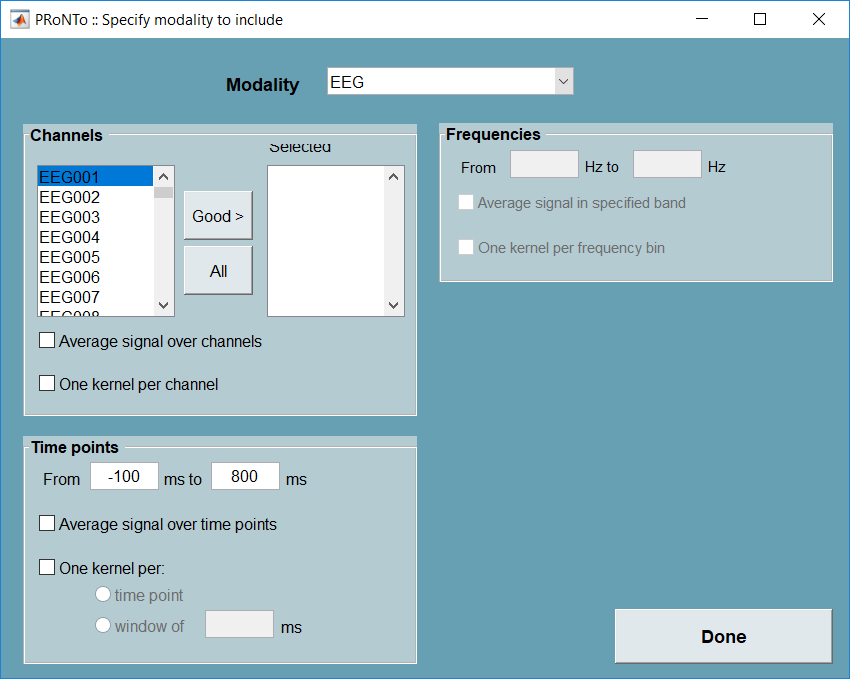
\includegraphics[height=9cm]{images/Tutorial/v3/gui_meeg_prepare_featureSet_specify_modality.png}
   \caption{`Specify modality' GUI for MEEG data.}
    \label{fig:gui_meeg_prepare_featureSet_specify_modality}
  \end{center}
\end{figure}


\subsubsection{Channels}

First of all, the user can play on the channels, selecting them all or only some, as well as average the signal over the selected channels, or build one kernel per channel. More specifically:

\begin{itemize}
\item The list of channels is displayed on the left panel, as unselected. To add a channel to the feature set, click on it. It will then appear on the right panel. Alternatively, you can select `All' channels or all `Good' channels. On Windows OS, the `bad' channels appear in red in the list.

\item \textbf{Average signal over channels:} this option will average the signal over all selected channels. This might be useful to obtain an average trace across a specific region of interest.

\item \textbf{One kernel per channel:} whether to build one kernel per channel (ticked) or not. This option corresponds to building an atlas with each channel as a `ROI'.
\end{itemize}





\subsubsection{Time points}

Similarly, the user can select a subset of the whole time window by specifying which time points (milliseconds) to extract features from. The signal can then be averaged over those time points, or the user could build one kernel per time point or one kernel per time window of a specified amount of milliseconds). More specifically:


\begin{itemize}
\item \textbf{Time window:} The time window is displayed and can be modified to include specific time points. When entering a value in milliseconds, PRoNTo will identify the closest corresponding time point.

\item \textbf{Average signal over time points:} The signal can be averaged across all selected time points.

\item \textbf{One kernel per:} One kernel can also be built, either per time point or per sub-windows of XX milliseconds (user-specified).

PRoNTo does not discard kernels when they have time points less than the user's specified time window, so to avoid big imbalances in the feature numbers across kernels you should ensure you provide the right window length. For example if you want to have 100ms subwindows between -100ms and 1100ms, the end time point should be 1099ms (because of the time point at 0ms). In this example, for balanced kernels, please specify the end of your global time window (here 1100) as the end time point desired minus your sampling interval in ms (here 1ms). So in that case the end of your global time window would be at 1099ms.

As a precautionary measure against a few time points ending up defining a whole kernel, whenever the defined global time window is not properly divisible by the defined time window, PRoNTo will automatically append the extra time points to the last kernel, if these extra time points account for less than 30\% of the defined time window, and will only create a new kernel to put the extra time points, if those are more than 30\%.
\end{itemize}









\subsubsection{Frequencies}

Finally, if the data set contain frequency information (i.e. multiple frequency bins), the user can select which bins to analyze, average the signal within the band of interest or build on kernel per frequency bin. More specifically:

\begin{itemize}

\item Similar to time points, the range of frequency bins included in the data can be viewed and specific sub-ranges selected.

\item \textbf{Average signal in specified band:} This is where the user can specify the frequency band to be averaged, as specified above. This is useful to test multiple frequency bands without having to manually perform the averages as a pre-processing step.

\item \textbf{One kernel per frequency bin:} This button will make PRoNTo build a kernel for each frequency bin.
\end{itemize}






\noindent \textbf{Note 1:} Features that are not present in the 1st file are greyed out and the corresponding panel cannot be accessed (e.g. frequencies in the present case).
\\

\noindent \textbf{Note 2:} It is not possible to average over one feature and select multiple kernels for that same feature (which is logical). It is however perfectly acceptable to build multiple kernels on more than one feature (e.g. one kernel per channel and per sub-time window of 50ms).
\\

The {\tt PRT.mat} structure saves all information linked to the file arrays in a {\tt fas} field (standing for `File Array Structure'), which size corresponds to the number of selected modality in all feature sets. The selected options and the link to the kernel (saved on the disk as a .mat) are stored in a {\tt fs} field (standing for `Feature Set'), which size corresponds to the number of feature sets defined by the user.
\\

\noindent \textbf{Important note:} When working with Graphical User Interfaces (GUIs), some messages might appear in \matlab{} workspace. These can display information about the operations currently performed or explain why the toolbox does not do as the user expected (e.g. when a file could not be loaded or if information was input in a wrong format). Therefore we strongly encourage the user to have a look at \matlab{} prompt when using GUIs.
\\

Finally, we want to remind the reader once more that in the main window, from PRoNTo v3.0 while it is still possible to concatenate multiple modalities (i.e. runs) in samples, it is NOT possible to build one kernel per modality anymore, as this functionality has been transferred to the model step.



\section{Batch interface}
\label{sec:matlabbatch_3_4}
%=======================

The `Feature set / Kernel' {\tt matlabbatch} module (Figure \ref{fig:batchFS}) allows the input/selection of all parameters and options aforementioned. Just note that the batch is based on the names of the modalities and/or conditions. Therefore, for the batch to work properly, names should be consistent across all steps, starting from data and design to the model specification and running. % The hierarchy for the case of a feature set containing one fMRI modality is displayed in (Fig. \ref{fig:batchFS}). For this feature set, we chose to load an atlas, and build multiple kernels based on the regions it defines.
\\

\begin{figure}[!h]
  \begin{center}
      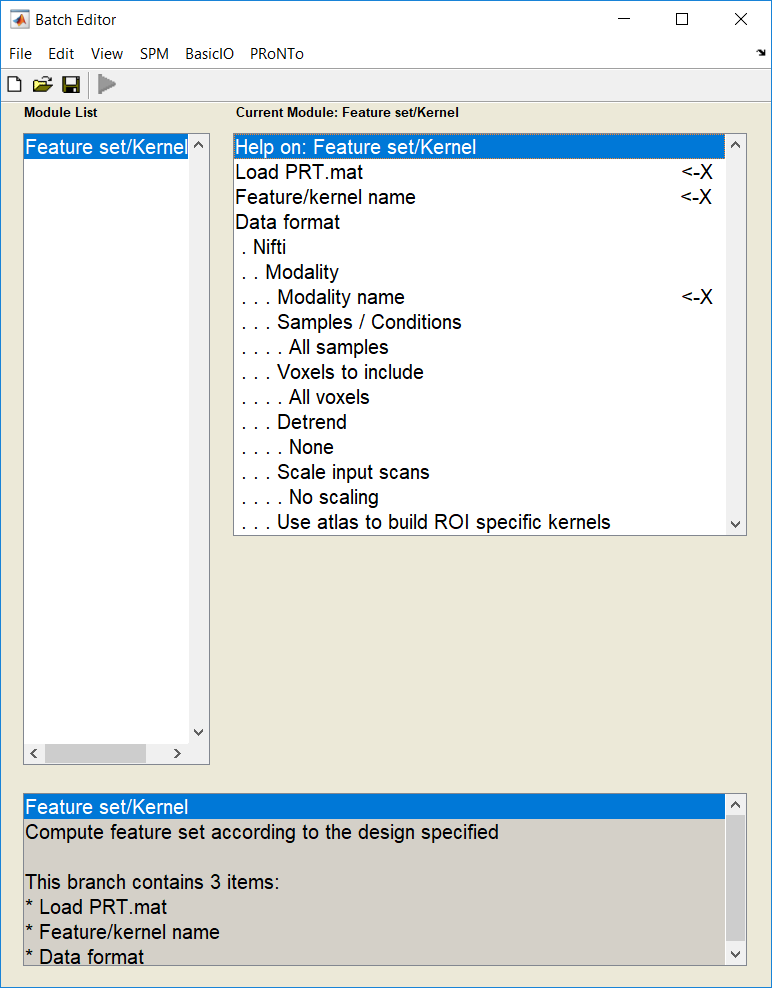
\includegraphics[height=10cm]{images/Tutorial/v3/prepare_feature_set_batch.png}
   \caption{{\tt matlabbatch} GUI for feature set building.}
    \label{fig:batchFS}
  \end{center}
\end{figure}

\noindent {\bf Important note:} Defining all important steps in one batch and running that batch will overwrite the {\tt PRT.mat} previously created and thus delete the links between the {\tt PRT.mat} and the computed kernel(s) and feature set(s). The file arrays would then be recomputed each time the batch is launched. For large datasets, we therefore recommend splitting the batch in two parts: a data and design and prepare feature set part and a second part comprising the model specification, run model and compute weights modules. This would indeed allow changing, e.g. model parameters, without recomputing the feature sets and kernels. 

% \vfill
% \vspace{30}

\section{PRT structure}

The PRT structure has been affected by these changes for the \textbf{fs} and \textbf{fas} structures (MEEG example):
\\

% \noindent \underline{\textbf{PRT.fs(1)}}

% \bi
% \item fs\_name: `TCChans'
% \item k\_file: `TCChans'
% \item id\_col\_names: {`group'  `subject'  `modality'  `condition'  `block'  `scan'}
% \item fas: [1x1 struct]
% \item modality: [1x1 struct]
% \item id\_mat: [550x6 double]
% \item multkernelROI: 1
% \item multkernel: 0
% \item atlas\_name: `Ch\_fr\_tp'
% \ei

% \noindent \underline{\textbf{PRT.fs(1).modality}}

% \bi
% \item mod\_name: {'ECoG'}
% \item aver: [0 0 0]
% \item multkern: [1 0 0]
% \item normalise: [1x1 struct]
% \item idfeat\_fas: [17199x1 double]
% \item dim\_m: {[49x1 double]  [1]  [1x351 double]}
% \item idfeat\_img: {49x1 cell}
% \item igood\_kerns: [1x49 double]
% \ei

In PRT.fs.modality, the fields `aver' and `multkern' were added. They represent which features averaging or multiple kernels were performed. This information is important for the construction of the weights later on. The `dim\_m' field also keeps the indexes of which channels, frequency bins and time points were used. Again, it is useful for the weights and the display of the weights (to obtain channel labels for example).
\\

Regarding the file array structure, the hdr is the object of the first file for the first subject of the modality. It allows to keep the channel labels, time points and frequency bins, as we would for image orientation or so. `idfeat\_img' is empty as it is not possible/useful to have a 1st level mask.
\\

% \noindent \underline{\textbf{PRT.fas}}

% \bi
% \item mod\_name: {`ECoG'}
% \item dat: [550x33696 file\_array]
% \item hdr: [96x351x550 meeg]
% \item idfeat\_img: []
% \ei



